%! Author = matt_dumont
%! Date = 4/12/23

\phantomsection % add to toc (make the link go to the right location)
\addcontentsline{toc}{section}{Executive Summary} % add to toc
\section*{Executive Summary} \label{exsum} % the asterisk prevents a section number from being assigned

\gls{pc1} of the Canterbury Land and Water Regional Plan included requirements for farmers in the Selwyn Waihora catchment to reduce nitrate discharges to groundwater to support water quality improvements.
\gls{pc1} became operational in 2016 with a requirement for \gls{no3n} reductions to be fully implemented by 2022.
Very few monitoring sites in the Selwyn Waihora catchment show decreasing \gls{no3n} concentrations to date.
This study evaluates the change detection power analysis of 56 sites (46 groundwater wells and 10 surface water features) to identify when and if \gls{pc1} reductions might become detectable in the current monitoring programme.

\begin{wrapfigure}{R}{0.70\textwidth}
    \begin{breakawaybox}[]{What is Detection Power}
        Essentially, detection power describes the chance that you can see what's really going on in the data.
        More specifically, detection power is the percent probability of detecting a statistically robust trend in the receptor concentration time series.
        Noisy data reduces the detection power while more frequent sampling increases the detection power.
        \\
        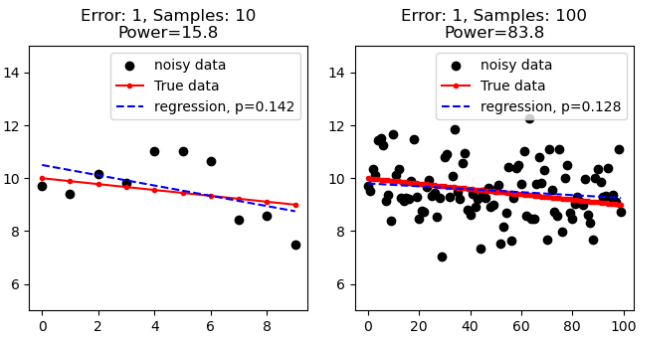
\includegraphics[width=0.95\textwidth]{figures/dp_ex_small}
    \end{breakawaybox}
\end{wrapfigure}

Our analysis suggests that the current monitoring programme is not well suited to detecting reductions in nitrate at the scale required by \gls{pc1}.
\gls{pc1} requires nitrate load reductions between 2-30\% depending on land use \autoref{box:no3_red}.
Here we assume at a 20\% reduction in nitrate loads is equivalent to a 20\% reduction in leachate nitrate concentrations; however changes in coincident land surface recharge (e.g., the move to efficient irrigation), could yield lower than expected reductions in nitrate leachate concentrations.
Our analysis suggests that approximately 60\% of groundwater monitoring sites will show decreasing \gls{no3n} concentrations (negative slope) if nitrate concentrations in source soil drainage water reduce by 10-20\%.
The remaining 40\% of sites are likely to plateau at a higher concentration than was recorded in 2016.
Note that these steady state concentrations will be lower than if \gls{pc1} had not been implemented.
The impact of \gls{pc1} on these \say{plateau} sites will not be detectable via slope monitoring(looking for a decreasing concentration trend), but future work may be able to detect these changes using a counter-factual approach.
There is significant uncertainty in these estimates due to the lack of \gls{mrt} data in c. 60\% of the groundwater monitoring locations we investigated.
However, if our \gls{mrt} estimates are correct then the nitrate reductions required under \gls{pc1} should be detectable in c. 30\% of the monitoring wells (50\% of those which can have a decreasing trend) by c. 2060.
Increasing sampling frequencies to monthly or weekly would allow detection of the reductions in c. 30\% of the monitoring wells by 2040 or 2035, respectively.

Surface water features generally receive water from a much larger catchment than individual wells and are therefore more likely to provide a landscape scale representative of policy and land management action effectiveness. However, no water age data are available for surface water courses in the Selwyn Waihora catchment making robust predictions of change detection power impossible.
We therefore derived detection power estimates by assuming a range of \gls{mrt} values.
Our results show that the detection power of the surface water features is highly sensitive to the assumed \gls{mrt} value.

Our analysis of Hart's creek highlights the uncertainty associated with our assumed water ages: results indicate that the maximum steady state \gls{no3n} concentration could be as low as 7.6 mg/l (assuming a \gls{mrt} of 5 years) or could be as high as 12.0 mg/l (assuming a \gls{mrt} of 30 years).
A stated goal of \gls{pc1} was to set an annual limit across all the shallow groundwater of not more than 8.5 mg/L.
The Hart's creek results may indicate that the \gls{pc1} reductions are sufficient to achieve this goal, or that the reductions are insufficient to prevent shallow groundwater from exceeding the \gls{mav}.
Obtaining age data for the surface water network would constrain these predictions and allow integrated analysis of detection power across the groundwater and surface water network.
The network could then be optimised in terms of the number and location of sites and monitoring frequency for change detection power, spatial representativeness and monitoring cost.
Age data collection for surface watercourses would also help to constrain the likely maximum \gls{no3n} concentration in a stream that will arise from current and past land use; this will provide a much clearer picture of policy and land management actions required to achieve water quality objectives.

We conclude that the current groundwater monitoring programme is unlikely to detect whether the nitrate reductions mandated under \gls{pc1} have improved water quality within the timeframes required for effective water resource management (within 30 years or less).
Previous analysis has focused on lag times as the key constraint on detecting change, but this analysis shows that statistical power is an equally important constraint under the current sampling frequency, which compounds the change detection limitations of the network.
We recommend that the change detection monitoring design framework described in the \textit{\href{https://github.com/Komanawa-Solutions-Ltd/gw_detect_power/blob/main/supporting_documents/Water_quality_monitoring_for_management_of_diffuse_nitrate_pollution_Final.pdf}{Water quality monitoring for management of diffuse nitrate pollution report}}\citep{olw_guidance}
should be applied to improve the surface water and groundwater monitoring programme for change detection. Key tasks will include:
\begin{itemize}
    \item Obtaining water age data for all key monitoring sites, particularly in surface water courses.
    \item Developing a basic conceptual model of the spatial distribution and rate of expected nitrate loss reductions, water flow paths, potential attenuation and travel times.
    \item Carrying out an integrated analysis of groundwater and surface water detection power for existing sites in the monitoring area using the information provided in this report, updated with new water age data where required, and identifying the highest detection power sites.
    \item Evaluating the representativeness of high power monitoring sites in relation to the expected spatial distribution and distribution of nitrate loss reductions and the number of sites required to confidently detect change.
    \item Identify new monitoring sites if existing network detection power and/or representativeness is inadequate.
    \item Undertaking a sampling frequency cost-benefit analysis.
    \item Undertaking more sophisticated statistical analysis to extract additional information from the existing data.
    \item Finalising network and monitoring design.
    \item Reviewing data after 1, 3 and 5 years of sampling to determine whether detection power and timeframe requirements have changed in light of new information.
\end{itemize}
We note that these recommendations will require a significant investment in monitoring infrastructure and data collection.  A companion study found that a 100-300\% increase in investment is likely required nationally to meet these goals \citep{dumont_determining_nodate}. This highlights the discrepancy between the goals of national monitoring programmes and the resources available to regional councils to meet these goals. This is a national challenge and cannot be ascribed as a failure of Environment Canterbury or any other regional council.

A key caveat of this report is that we only focused on one aspect of the monitoring programme: detecting changes in \gls{no3n} concentrations. The network serves and was primarily designed for multiple other purposes some of which are counter to high detection powers (e.g., characterising the state of the deep aquifer system). We also have not assessed the spatial representativeness of the monitoring network in this analysis (for either change detection or more broadly) as it was beyond the scope of this project.